\documentclass[journal]{IEEEtran}
\usepackage{amsmath}    % Para fórmulas matemáticas
\usepackage{amssymb}    % Para símbolos matemáticos adicionales
\usepackage{amsfonts}   % Para fuentes de matemáticas
\usepackage{graphicx}   % Para incluir imágenes
\usepackage{subcaption}
\usepackage{cite}       % Para gestionar las citas bibliográficas
\usepackage{booktabs}   % Para tablas con líneas profesionales
\usepackage{multirow}   % Para celdas de múltiples filas en tablas
\usepackage{float}      % Para mejor control de la ubicación de las figuras
\usepackage[utf8]{inputenc}
\usepackage[T1]{fontenc}
\usepackage{booktabs,siunitx,makecell,multirow,tabularx}
\usepackage[para,online,flushleft]{threeparttable}
\sisetup{
	group-separator = {\,},   
	group-minimum-digits = 4,
	output-decimal-marker = {.}
}

\title{ CO$_{2}$ classification analysis for AI models}

\author{
	\IEEEauthorblockN{Juan Felipe Gallo Rendón\IEEEauthorrefmark{1}}
	\IEEEauthorblockA{\textit{Engineering department} \\
		\textit{University of Antioquia}\\
		Medellín, Colombia}
}

\begin{document}
	\maketitle

	\begin{abstract}

	\end{abstract}

	\begin{IEEEkeywords}
		Cluster analysis, K-means, Classification models, 
	\end{IEEEkeywords}


	\section{Introduction}



	\section{Methodology}
	\label{sec:methodology}
	Classification methods are applied to the selected dataset. A workflow comprising $six$ procedures is followed: \textbf{univariate analysis}, \textbf{cluster analysis}, \textbf{k-means clustering}, \textbf{linear classification}, and \textbf{nonlinear classification}. Upon completion of these steps, the results are compared and the best-performing model is identified.

	\subsection{Univariate Analysis}
	In this stage, the dataset \textbf{HFCO2.csv}—originating from a $\text{CO}_2$-emissions report on the Hugging Face platform—is profiled to characterize marginal distributions, identify outliers, and screen variables for subsequent modeling. The variables under study are enumerated below. Variables such as \texttt{modelId}, \texttt{datasets}, \texttt{co2\_reported}, \texttt{createdat}, and \texttt{libraryname} are excluded due to limited analytical relevance; \texttt{database\_efficiency} is removed because it is functionally dependent on \texttt{co2\_eq\_emissions} and \texttt{size}.
	Because no native target is present, classification labels are defined to enable supervised evaluation. First, \texttt{model\_type} is created to align the \texttt{performance\_score} with the appropriate metric family (e.g., accuracy, F1, Rouge); rows lacking performance metrics are discarded. Univariate summaries and frequency counts are then computed for qualitative variables (e.g., \texttt{model\_type}) and proportions are reported for \texttt{domain}; variables exhibiting near-constant distributions (e.g., \texttt{library\_name} = \texttt{pytorch}), or extreme sparsity (\texttt{geographical\_location}, \texttt{environment}) are removed.
	Finally, a fairness-oriented label is introduced to relate predictive performance to environmental impact, yielding four categories—\emph{Fair and Efficient}, \emph{Powerful but Expensive}, \emph{Green but Weak}, and \emph{Inefficient}—and a derived Boolean variable \texttt{is\_fair}. The resulting curated dataset and label structure provide the basis for the next methodological step, cluster analysis.


	\subsection{Cluster analysis}
	\label{methodology:cluanal}
	A hierarchical clustering analysis was applied to segment AI models using numeric performance-and-cost variables. Records with N/A/$\infty$ were removed and features were were standardized to z-scores, to mitigate dominance of high skewed counts in features like \texttt{downloads} and \texttt{likes}, simple transformation (log/winsorzing) were considered. Two distances were evaluated: Euclidean and Mahalanobis, the latter computed with a Ledoit-Wold covariance estimator. Four linkage rules (Ward, average, complete and single) were compared.
	The dendogram was cut either at a target k (k $\in{\{3,4\}}$) to improve size balance or at the k that maximized the average silhouette; the equivalent distance threshold reproducing that partition was also recorded. Internal quality was assessed with the silhouette score, while cophenetic correlation was used descriptively to gauge dendogram fidelity. As external validation, labels (\texttt{is\_fair}, \texttt{fairness\_class}, \texttt{model\_type}) were not used for training and were cotrasted post-hoc via contingency tables, $\chi$²/Crammer's V, and adjusted Rand index.
	Cluster interpretation relied on profiles in original units and on z-centroids; a |z| ranking highlighted the most discriminative variables. A comparative summary across configurations (metrics, thresholds, balance) and visualizations (dedongrams with horizontal cut, stacked proportions and heatmaps) were produced for review.Final selection prioritized overall separability and operational usefulness, balancing silhouette with stability, cluster-size balance and consistency with external labels. 

\subsubsection*{K-means analysis}
K-means was applied to the same numeric variables used in the hierarchical analysis
(\textit{performance\_score}, \textit{co2\_eq\_emissions}, \textit{likes}, \textit{downloads}, \textit{size}).
Rows with non-numeric/inf values were removed and features were standardized to $z$-scores
(\texttt{StandardScaler}). We explored $k\in\{2,\ldots,10\}$ with \texttt{k-means++}
initialization ($n\_init=50$, \texttt{max\_iter}=500, \texttt{random\_state}=42).

For each $k$ we reported: Silhouette (higher is better), Calinski–Harabasz (CH; higher is better),
Davies–Bouldin (DBI; lower is better), and the inertia (\emph{elbow} curve).
The primary selector was the maximum Silhouette; CH/DBI and the elbow were used as
secondary evidence.

For the selected $k$ we exported cluster sizes, original-unit profiles (count/mean/median),
$z$-centroids, and a variable ranking using $\max|z|$ (to highlight the most discriminative features).
External labels (\textit{is\_fair}, \textit{clasification\_fairness}, \textit{model\_type})
were held out from training and only used for validation via contingency tables,
$\chi^2$/Cramér’s $V$, Fisher’s exact test when $2\times 2$, and ARI when applicable.


\subsection{Multivariate Normality \& LDA Feasibility — Methods}
\label{sec:method-lda}

Check whether the feature vector
X=\texttt{performance\_score}, \texttt{co2\_eq\_emissions}, \texttt{likes}, \texttt{downloads}, \texttt{size}
is (approximately) multivariate normal—globally and within classes—so that classical LDA is justified.

\textbf{Preprocessing.} Remove rows with NA/inf; standardize all variables to $z$–scores.

\textbf{Robust scatter \& distances.} Fit a shrinkage (Ledoit–Wolf) covariance
$\widehat{\Sigma}$ to mitigate outliers. Compute squared Mahalanobis distances
$d_i^2=(x_i-\widehat{\mu})^\top\widehat{\Sigma}^{-1}(x_i-\widehat{\mu})$ (i) globally and
(ii) per class.

\textbf{Normality diagnostic.} Under MVN with $p$ variables, $d_i^2\sim\chi^2_p$.
Compare empirical quantiles of $\{d_i^2\}$ against $\chi^2_p$ using QQ–plots:
global and class–conditional. Large, systematic upward deviations (heavy tails/mixtures) indicate
non–normality.

\textbf{Optional formal checks.} (a) Mardia or Henze–Zirkler tests on $z$–scores; (b) Box’s $M$
(or visual comparison) for equality of class covariances.

\textbf{Decision rule.}
\begin{enumerate}[nosep,leftmargin=*]
	\item \emph{Proceed with classical LDA} if QQ–plots track the $\chi^2_p$ line reasonably well
	(globally \emph{and} by class) and class covariances appear similar.
	\item \emph{Prefer robust/regularized LDA or nonparametric classifiers}
	(e.g., shrinkage LDA, logistic regression, tree–based) if tails inflate, classes differ in
	scatter, or tests reject MVN/homoscedasticity.
\end{enumerate}

\subsection{LDA }

Multivariate normality was examined via Mahalanobis Q–Q diagnostics (globally and by class). Because clear departures from normality were observed, regularized discriminants were preferred. Linear Discriminant Analysis (LDA) with automatic shrinkage (and, for projections, the \texttt{eigen} solver) and Quadratic Discriminant Analysis (QDA) with mild regularization were fit on a stratified train/test split. Performance was summarized with confusion matrices, precision/recall/F1, ROC–AUC, and 5–fold stratified cross–validation. Model parameters (priors, class means, coefficients, scalings), LD scores, and plots (ROC, score histograms, dendrograms) were exported to files to enable reporting and reproducibility.

\subsection{Non-linear models comparison)}
A supervised classification workflow was implemented to benchmark a linear baseline
(Linear Discriminant Analysis, LDA) against two non-linear alternatives:
an RBF–kernel Support Vector Machine (SVM–RBF) and Gradient Boosting (GB).
The target was the binary label \texttt{is\_fair}; predictors were the numeric
performance–cost variables used in previous sections. Missing values were removed,
then features were transformed with $\log(1+x)$ (for skewed counts: CO$_2$, likes,
downloads, size) and standardized (zero mean, unit variance). A stratified
train/test split (70/30) preserved the empirical class imbalance. 

Models were trained in scikit-learn as follows.
LDA used the \texttt{eigen} solver with automatic shrinkage, providing a robust
shared covariance estimate and interpretable discriminant directions. SVM–RBF used
probability calibration (\texttt{probability=True}) and an RBF kernel; GB used
logistic loss with modest depth and learning rate (standard defaults), both selected
via stratified 5-fold cross-validation (CV) on the training fold. Evaluation focused
on rank-based and decision-based criteria: AUC(ROC), average precision (AP) for the
positive class (\emph{True}), F1 for the positive class, overall accuracy, and
Brier score (probability calibration). Error structure was inspected through
confusion matrices. For comparability, models were scored on the same held-out test
set; CV accuracy was also reported to assess stability across resamples. Curves
(ROC and Precision–Recall) and panels (confusion matrices) were produced for visual
diagnostics and threshold selection.
	\section{Results and discussions}

	\label{sec:results}
LOREMPIPSUM

	 \subsection{Univariate Analysis}
	 \label{ssec:unianal}
	 The database \textbf{HFCO2.csv} is a product of the $\text{CO}_2$ emissions report generated on the Hugging Face platform. In this case, the analysis is focused on the following variables:

	 \begin{enumerate}
	 	\item[]\hspace{-\labelwidth}\hspace{-\labelsep}
	 	\item \texttt{co2\_eq\_emissions}: the resulting carbon footprint
	 	\item \texttt{downloads}: number of model downloads
	 	\item \texttt{likes}: number of model likes
	 	\item \texttt{performance\_metrics}: (accuracy, F1, Rouge-1, Rouge-L)
	 	\item \texttt{performance\_score}: the harmonic mean of the normalized performance metrics
	 	\item \texttt{size}: size of the final trained model in MB
	 \end{enumerate}
	 Variables like \texttt{modelId}, \texttt{datasets}, \texttt{co2\_reported}, \texttt{createdat}, and \texttt{libraryname} were removed because of their lack of importance in the analysis. \texttt{database\_efficiency} was also removed because it is a dependent variable of \texttt{co2\_eq\_emissions} and \texttt{size}.
	 The first step was to choose metrics for classification, as the database \textit{per se} does not have a relevant dependent variable to be classified. Therefore, some labels were created with the aim of creating a dependent variable to be predicted by a couple of machine learning models. Accordingly, \texttt{model\_type} is the label used to determine which metric the model uses for its performance score, because not all models use the same metric for evaluation. After applying this classification, some rows were unusable because hundreds of them do not have performance metrics at all, so they were deleted.
	 After the redundant rows were erased, a count was made on the qualitative variables, as shown in the following table:



	 \begin{table}[H]
	 	\centering
	 	\caption{model\_type counts}
	 	\begin{tabular}{l c }
	 		\toprule
	 		model type & count \\
	 		\midrule
	 		type1 (accuracy \& f1)  & 773 \\
	 		type2 (rouge)           & 228 \\
	 		type3 (accuracy)        & 72 \\
	 		type4 (rouge1)          & 3 \\
	 		type5 (f1)   			& 2 \\
	 		\bottomrule
	 	\end{tabular}
	 	\label{tab:model_type_counts}
	 \end{table}

	 In an effort to find relationships between model types and the other categories, a summary of the other variables was prepared, focusing on the \texttt{domain} variable, which is the model's use case. The following table shows each domain and the associated percentage:
	 \begin{table}[H]
	 	\centering
	 	\caption{percentage of domains}
	 	\begin{tabular}{l c }
	 		\toprule
	 		model type & count \\
	 		\midrule
	 		NLP  & 81,5\% \\
	 		Computer Vision & 16,0\% \\
	 		Not specified        & 2,5\% \\
	 		\bottomrule
	 	\end{tabular}
	 	\label{tab:domain_percentage}
	 \end{table}
	 In conclusion, there are only two major types of domain models. For the purpose of this analysis, this is not an influential variable, so it was removed.
	 Other variables, like \texttt{library\_name}, revealed that all models use \texttt{pytorch} as a library, so this was also removed. The same reasoning applied to \texttt{geographical\_location}: the analysis revealed that 99\% of the models do not specify the training location. Similarly, 99.7\% of the models do not report the hardware used in \texttt{environment}.
	 After applying analysis upon the mean of performance metrics and $\text{CO}_2$ emissions, the analysis revealed that those models could be labeled again with a more precise metric: \textit{fairness}, defined as a relation between performance score and $\text{CO}_2$ emissions. The following are the labels chosen for the models
	 \begin{enumerate}
	 	\item[]\hspace{-\labelwidth}\hspace{-\labelsep}
	 	\item Fair and Efficient
	 	\item Powerful but Expensive
	 	\item Green but Weak
	 	\item Inefficient
	 \end{enumerate}

	 Finally, models were classified by a new boolean variable "is\_fair", and those that were previously labeled with respective performance metrics, were evaluated:
	 \begin{table}[htbp]
	 	\centering
	 	\caption{Model Classification based on their fairness and performance metrics}
	 	\label{tab:clasificacion_modelos}
	 	\begin{tabular}{l l r}
	 		\toprule
	 		\textbf{Model Type} & \textbf{Classification Fairness} & \textbf{Count} \\
	 		\midrule

	 		\multirow{5}{*}{\shortstack{type1\\ (accuracy \& f1)}} & Fair and Efficient & 229 \\
	 		& Powerful but Expensive & 214 \\
	 		& Green but Weak & 181 \\
	 		& Inefficient & 142 \\
	 		& Incomplete data & 7 \\
	 		\midrule

	 		\multirow{5}{*}{\shortstack{type2\\ (rouge)}} & Inefficient & 140 \\
	 		& Green but Weak & 57 \\
	 		& Powerful but Expensive & 18 \\
	 		& Fair and Efficient & 9 \\
	 		& Incomplete data & 4 \\
	 		\midrule

	 		\multirow{5}{*}{\shortstack{type3\\ (accuracy)}} & Fair and Efficient & 50 \\
	 		& Powerful but Expensive & 9 \\
	 		& Green but Weak & 7 \\
	 		& Incomplete data & 4 \\
	 		& Inefficient & 2 \\
	 		\midrule

	 		\multirow{2}{*}{\shortstack{type4 (f1)}} & Incomplete data & 2 \\
	 		& &  \\
	 		\midrule

	 		\multirow{2}{*}{\shortstack{type5 (rouge1)}} & Incomplete data & 3 \\
	 		& &  \\
	 		\bottomrule
	 	\end{tabular}
	 \end{table}
	 Results are consigned in the route: \texttt{/notebooks/part2/1-univarated-analysis.ipynb}
	 Those classifications are required for the next step in the methodology, Cluster analysis.


\subsection{Cluster Analysis}

A grid over \emph{distance} $\times$ \emph{linkage} found that the highest internal separation was achieved by
\textbf{Single–Euclidean} with \textbf{$k=3$} (silhouette $\approx 0.62$, cophenetic $\approx 0.71$). Close contenders were
\emph{Complete–Mahalanobis} ($k=3$, silhouette $\approx 0.52$, cophenetic $\approx 0.71$) and
\emph{Average–Mahalanobis} ($k=3$, silhouette $\approx 0.43$, cophenetic $\approx 0.81$).
Among the “non-single” options, \textbf{Average–Euclidean} with \textbf{$k=4$} offered a more conservative structure
(silhouette $\approx 0.34$, cophenetic $\approx 0.81$). \emph{Ward–Euclidean} showed the lowest separation
(silhouette $\approx 0.20$, cophenetic $\approx 0.44$).

\begin{figure}[H]
	\centering
	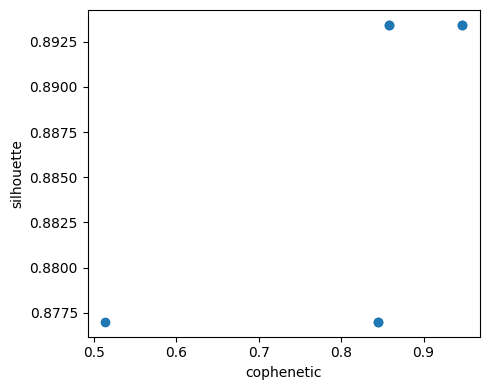
\includegraphics[width=0.8\columnwidth]{assets/1_coph_vs_silhouette.png}
	\caption{Cophenetic vs.\ silhouette for all configurations. Top-right indicates better fidelity and separation.}
	\label{fig:coph_vs_silhouette}
\end{figure}

Because \emph{single} linkage may form chaining clusters, we report two complementary views:
(i) the best-silhouette solution (\textbf{Single–Euclid, $k=3$}) and (ii) a robust alternative without single linkage
(\textbf{Average–Euclid, $k=4$}). The horizontal cut at the recorded equivalent threshold reproduces the same $k$ in the
dendrogram.

\begin{figure}[H]
	\centering
	% Replace with the dendrogram you want as the main figure
	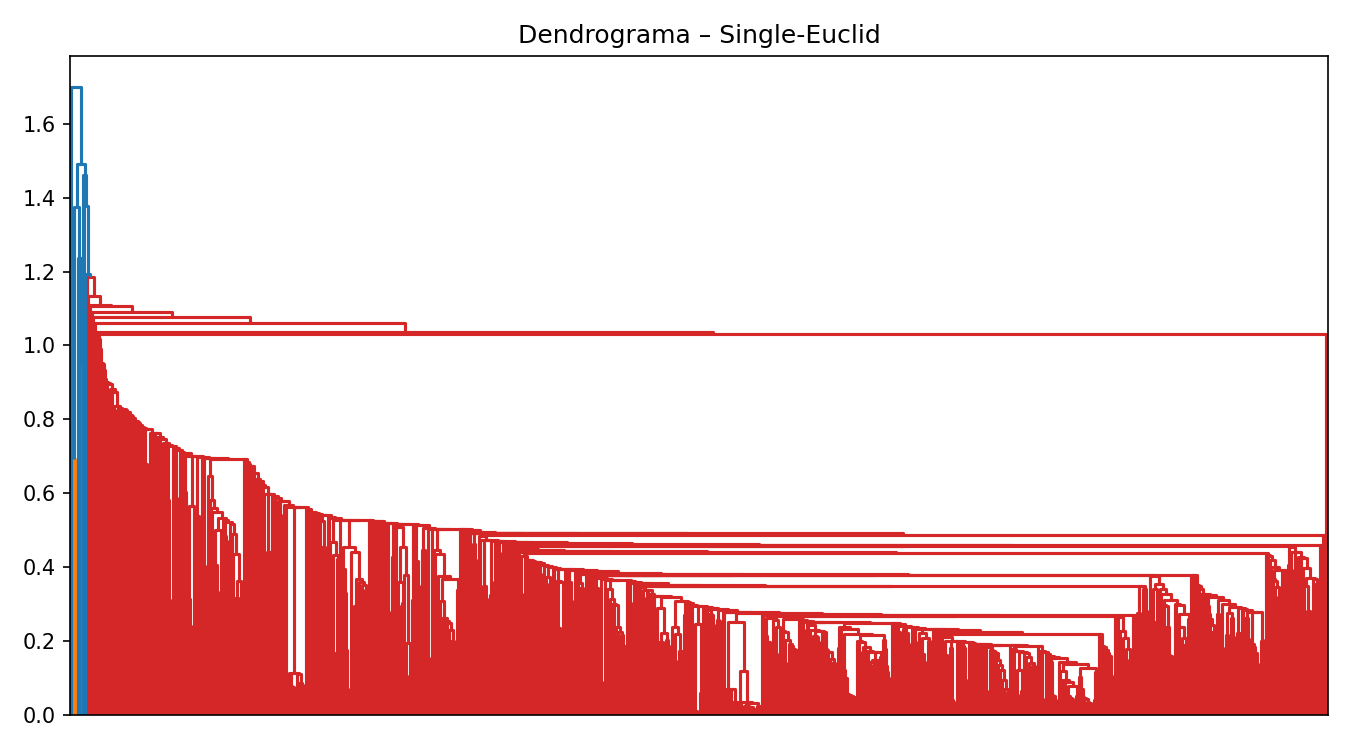
\includegraphics[width=0.8\columnwidth]{assets/4_dendogram_single.png}
	\caption{Dendrogram—Single–Euclidean. The horizontal cut at the equivalent threshold yields $k=3$.}
	\label{fig:dendro_single_euclid}
\end{figure}

Across configurations, a \emph{dominant} “catalog” cluster concentrates the bulk of models near global means, while
1–3 \emph{small} “elite” clusters group items with markedly higher \emph{downloads/likes/performance} and (on average)
lower \emph{size/CO\textsubscript{2}}. Variable importance from $z$–centroids is consistent: the most discriminative
feature is \textbf{downloads} (max $|z|\approx 5.39$), followed by \textbf{likes} ($\approx 2.03$), then
\emph{CO\textsubscript{2}} and \emph{performance} (moderate), with \emph{size} contributing less ($\approx 1.32$).

External validation against labels was limited, as expected (labels were not used to train the clustering):
ARI vs.\ \texttt{is\_fair} stayed near zero across settings; however, cluster–label contingency showed reasonable
purities (mean $\sim 0.73$–$0.90$ depending on the configuration), with \texttt{is\_fair=True} enriched in one of the small
clusters and scarce in the large catalog group.

% --- Suggested figures for the chosen config ---
\begin{figure}[H]
	\centering
	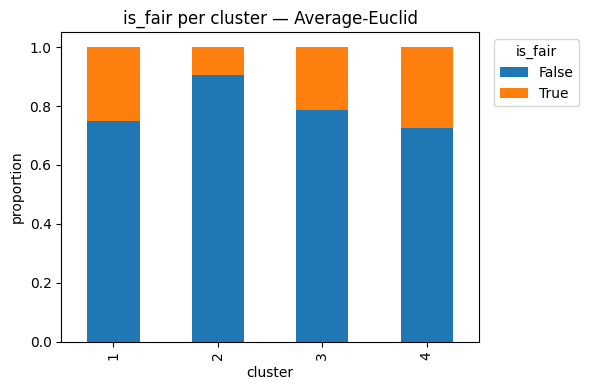
\includegraphics[width=0.8\columnwidth]{assets/3_is_fair_per_cluster.png}
	\caption{Stacked proportions of \texttt{is\_fair} per cluster (Average–Euclid, $k=4$).}
	\label{fig:isfair_stacked}
\end{figure}


\paragraph{Cluster profiles.}
Tables~\ref{tab:profile-a}–\ref{tab:profile-c} report \emph{original-unit} profiles (count/mean/median) for
\textit{performance\_score}, \textit{co2\_eq\_emissions}, \textit{likes}, \textit{downloads} and \textit{size}. For brevity,
we include the robust alternative (\emph{Average–Euclid, $k=4$}); the $z$–centroids and the $|z|$ ranking (downloads $\to$ likes)
appear in the Supplement.
\begin{table}[H]
	\centering
	\small
	\caption{Cluster profiles (original units): performance and CO$_2$}
	\label{tab:profile-a}
	\renewcommand{\arraystretch}{1.1}
	\begin{tabular}{l S[table-format=4.0] S[table-format=1.3] S[table-format=1.3]
			S[table-format=2.3] S[table-format=1.3]}
		\toprule
		& \multicolumn{3}{c}{\textbf{performance\_score}}
		& \multicolumn{2}{c}{\textbf{co2\_eq\_emissions}} \\
		\cmidrule(lr){2-4}\cmidrule(lr){5-6}
		\textbf{cluster} & \textbf{n} & \textbf{mean} & \textbf{median}
		& \textbf{mean} & \textbf{median} \\
		\midrule
		1 & 4    & 0.988 & 0.991 & 49.974 & 3.189 \\
		2 & 1029 & 0.727 & 0.822 & 71.382 & 2.749 \\
		\bottomrule
	\end{tabular}
\end{table}

\begin{table}[H]
	\centering
	\small
	\caption{Cluster profiles (original units): likes and downloads}
	\label{tab:profile-b}
	\renewcommand{\arraystretch}{1.1}
	\begin{tabular}{
			l
			S[table-format=4.0]        % n
			S[table-format=1.3]        % likes mean
			S[table-format=1.3]        % likes median
			S[table-format=6.2]        % downloads mean
			S[table-format=7.2]        % downloads median
		}
		\toprule
		& \multicolumn{3}{c}{\textbf{likes}}
		& \multicolumn{2}{c}{\textbf{downloads}} \\
		\cmidrule(lr){2-4}\cmidrule(lr){5-6}
		\textbf{cluster} & \textbf{n} & \textbf{mean} & \textbf{median}
		& \textbf{mean} & \textbf{median} \\
		\midrule
		1 & 4    & 2.250 & 0.500 & \num{104439.25} & \num{102572.50} \\
		2 & 1029 & 0.181 & 0.000 & \num{65.245}    & \num{5.00} \\
		\bottomrule
	\end{tabular}
\end{table}


\begin{table}[H]
	\centering
	\small
	\caption{Cluster profiles (original units): size ($\times 10^{8}$)}
	\label{tab:profile-c}
	\renewcommand{\arraystretch}{1.1}
	\begin{tabular}{l S[table-format=4.0] S[table-format=1.3] S[table-format=1.3]}
		\toprule
		\textbf{cluster} & \textbf{n} & \textbf{mean} & \textbf{median} \\
		\midrule
		1 & 4    & 2.649 & 2.654 \\
		2 & 1029 & 8.953 & 4.987 \\
		\bottomrule
	\end{tabular}
\end{table}

\paragraph{Overall quality.}
Across linkages and distances, the highest internal separation was obtained by \emph{Single–Euclid} with $k=3$
($\text{silhouette}\approx 0.62$, $\text{cophenetic}\approx 0.71$), followed by \emph{Complete–Mahalanobis}
($\text{silhouette}\approx 0.52$). Average-based variants trailed behind
($\text{silhouette}\approx 0.30$–$0.44$) and \emph{Ward–Euclid} showed the lowest separation
($\text{silhouette}\approx 0.20$).

\paragraph{Cluster profiles (what differentiates groups).}
Tables~\ref{tab:profile-a}–\ref{tab:profile-b} report original-unit profiles for a robust
reference solution. Consistent with the winning configuration, a small cluster concentrates very high
\emph{downloads}/\emph{likes} (and comparatively lower \emph{size}/CO$_2$), while a large “catalog” cluster
sits near the global mean. In $z$–space, \emph{downloads} shows the largest between-cluster contrast
($\max|z|\approx 5.39$), followed by \emph{likes} ($\approx 2.03$); CO$_2$, performance and size contribute
more modestly ($\approx 1.3$–$1.7$).

\paragraph{External validation (not used for training).}
Contingency tables indicate a small–to–moderate association between clusters and external labels.
For \emph{Single–Euclid} ($k=3$), the largest cluster concentrates the majority of \emph{is\_fair=False}
(share of \emph{True} $\approx 0.27$), whereas minor clusters show either higher \emph{True} share or are too small
to be conclusive.  (mean/weighted),
$\chi^{2}$ with Cramér’s $V$ ($\approx 0.03$–$0.07$ across configs), and Fisher’s exact test when applicable,
together with ARI vs.~\emph{is\_fair} (near zero, as expected for weak alignment).
Figure~\ref{fig:isfair_stacked} visualizes the \emph{is\_fair} proportions per cluster.

\paragraph{Sensitivity and limitations.}
The pattern is robust across $k\in[2,6]$ and across distance/linkage families that avoid overly compact
(\emph{ward}) or overly chained (\emph{single}) artifacts; nonetheless, cluster sizes remain unbalanced and
the \emph{single} linkage can induce chaining in dense regions. These caveats do not affect the substantive
finding that \emph{downloads} (and, secondarily, \emph{likes}) drive the segmentation.

 \subsection{Univariate Analysis}
We ran k-means on the standardized variables
(\textit{performance\_score}, \textit{co2\_eq\_emissions}, \textit{likes}, \textit{downloads}, \textit{size})
for $k\in\{2,\ldots,10\}$ with \texttt{k-means++}, $n_{\text{init}}{=}50$, \texttt{max\_iter}{=}500.
Model selection combined four internal criteria:

\begin{itemize}
	\item \textbf{Silhouette (max is best).} The curve peaked at $\mathbf{k=2}$ with $\approx\mathbf{0.286}$, and decreased thereafter (Fig.~\ref{fig:silhouette-kmeans}).
	\item \textbf{Calinski--Harabasz (max is best).} The maximum occurred at $k{=}3$ ($\approx\!330$), with $k{=}2$ close behind ($\approx\!290$) (Fig.~\ref{fig:ch-kmeans}).
	\item \textbf{Davies--Bouldin (min is best).} DBI decreased monotonically with $k$, reaching $\approx\!1.21$ at $k{=}10$ (Fig.~\ref{fig:dbi-kmeans}).
	\item \textbf{Elbow (inertia).} Inertia dropped rapidly up to $k{\sim}6$ and then flattened, with no sharp elbow afterwards (Fig.~\ref{fig:elbow-kmeans}).
\end{itemize}

Given the primary criterion (silhouette), we selected $\mathbf{k=2}$.
The resulting partition produced \textbf{unbalanced cluster sizes} (about $n{\sim}740$ vs.\ $n{\sim}300$; Fig.~\ref{fig:sizes-k2}).
Cluster profiles (in original units) and $z$–centroids were computed; the ranking by $\max|z|$ again highlighted
\textit{downloads} as the most discriminative variable, followed by \textit{likes}, with the remaining variables contributing less.
Cross-tabs against the external labels (\textit{is\_fair}, \textit{clasification\_fairness}, \textit{model\_type}) were generated for $k{=}2$
(see Supplement for the full tables).


\begin{figure}[H]
	\centering
	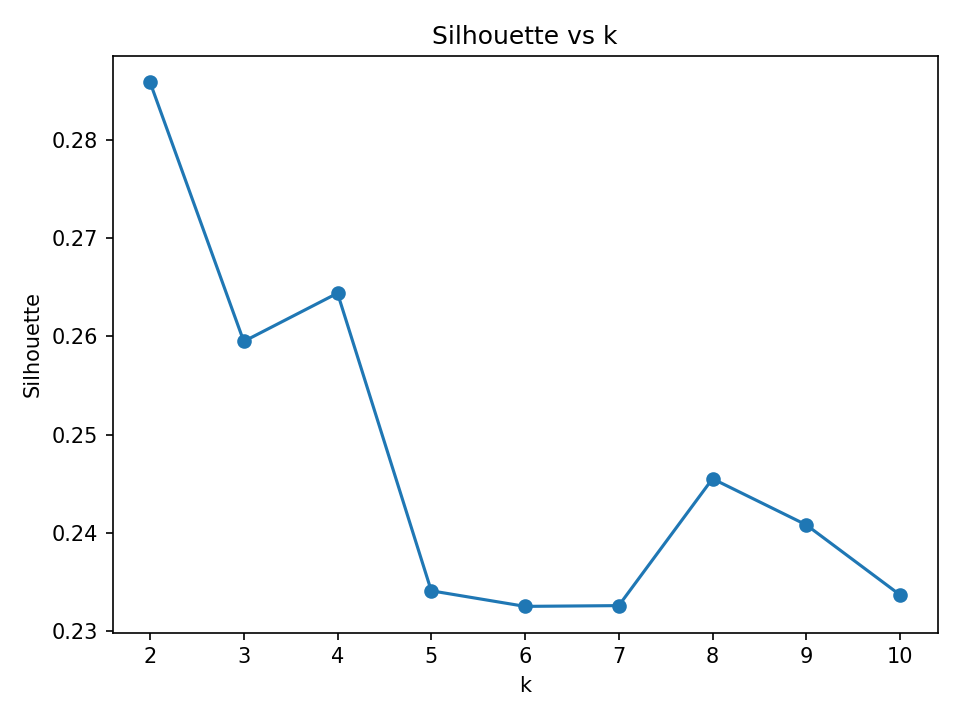
\includegraphics[width=.48\linewidth]{assets/silhouette_vs_k.png}\hfill
	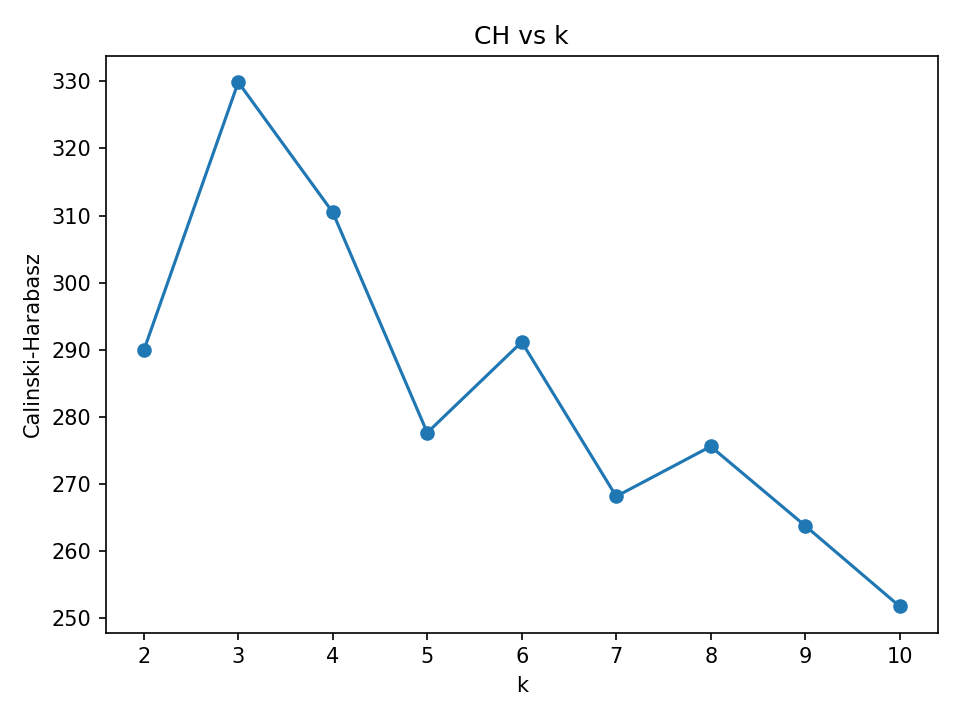
\includegraphics[width=.48\linewidth]{assets/ch_vs_k.png}
	\caption{Silhouette and Calinski--Harabasz across $k$.}
	\label{fig:silhouette-kmeans}\label{fig:ch-kmeans}
\end{figure}

\begin{figure}[H]
	\centering
	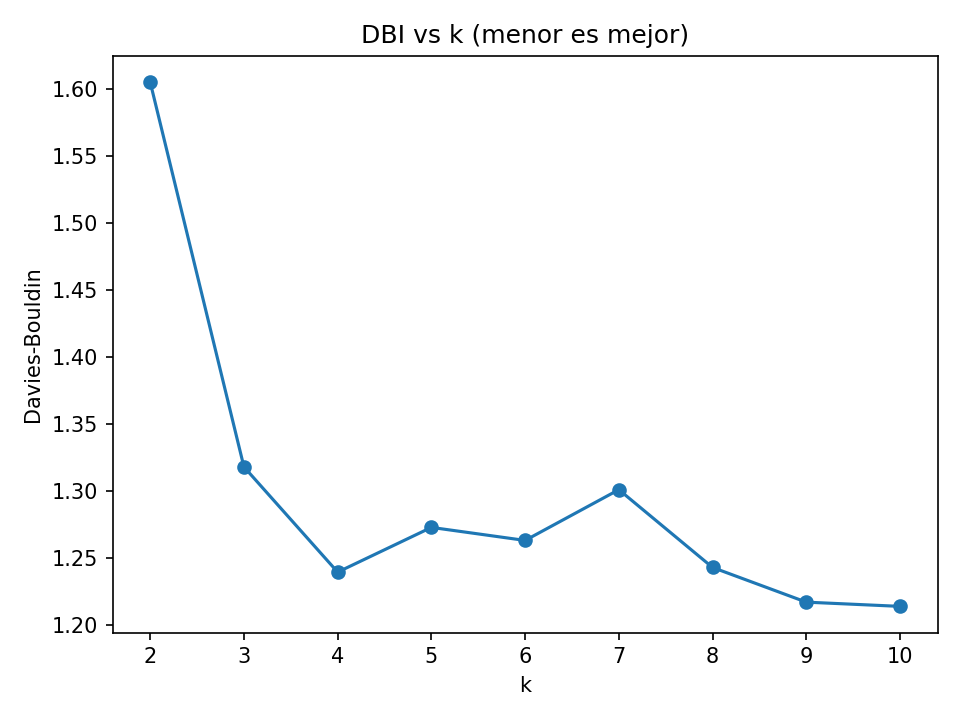
\includegraphics[width=.48\linewidth]{assets/dbi_vs_k.png}\hfill
	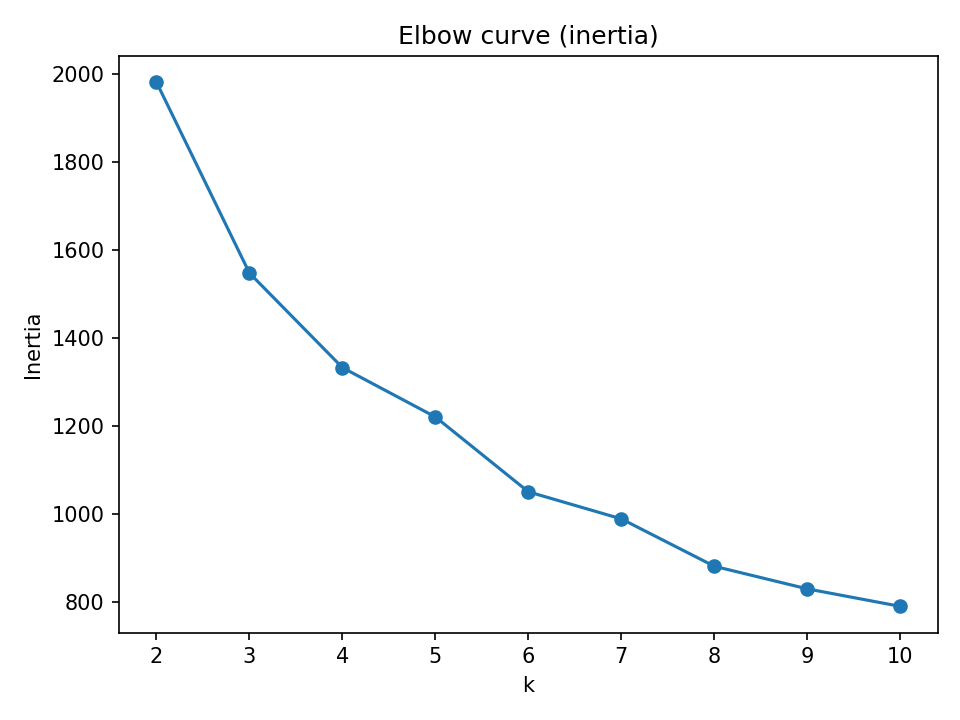
\includegraphics[width=.48\linewidth]{assets/elbow_inertia.png}
	\caption{Davies--Bouldin (lower is better) and inertia (elbow) across $k$.}
	\label{fig:dbi-kmeans}\label{fig:elbow-kmeans}
\end{figure}

\begin{figure}[H]
	\centering
	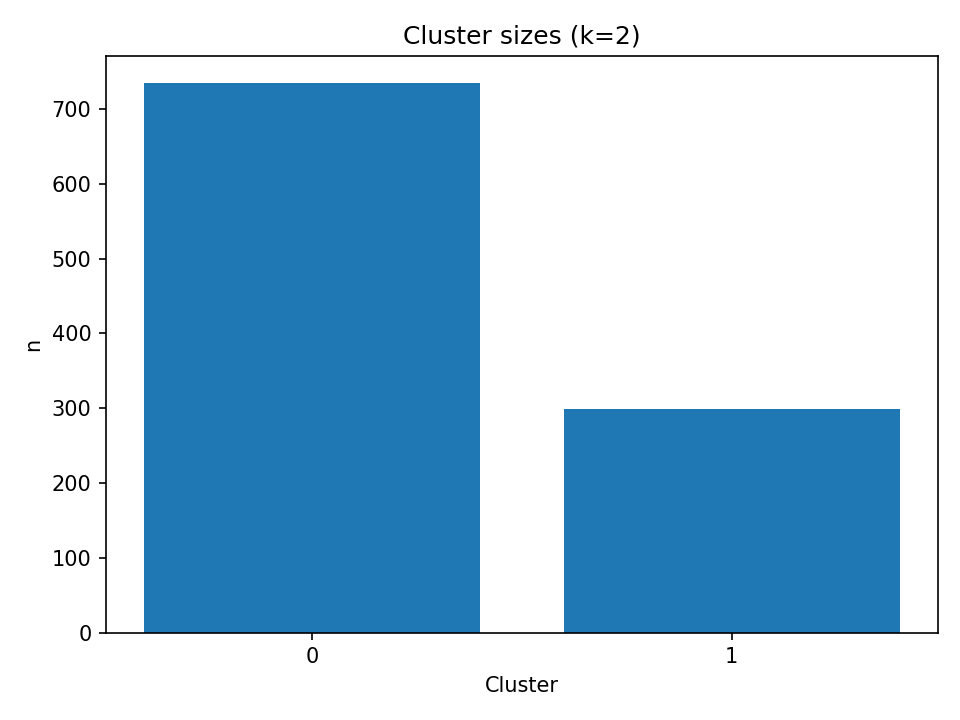
\includegraphics[width=.55\linewidth]{assets/cluster_sizes_k2.png}
	\caption{Cluster sizes for the selected solution ($k{=}2$).}
	\label{fig:sizes-k2}
\end{figure}
The internal criteria point to different trade-offs:
silhouette clearly favors \textbf{$k{=}2$}, Calinski--Harabasz prefers \textbf{$k{=}3$},
and Davies--Bouldin keeps improving as $k$ grows. In this context, we prioritized
silhouette because it balances compactness and separation and is less biased by the growth
of $k$ than CH/DBI. The \emph{elbow} curve shows diminishing returns beyond $k{\sim}6$,
supporting the choice of a small number of groups.

The $k{=}2$ solution is \emph{interpretable} and \emph{stable} (across restarts) but
\emph{unbalanced}: one major segment (catalog-like) and a smaller, high-intensity segment.
The profile tables indicate that the minor cluster concentrates substantially higher
\emph{downloads} and \emph{likes} (and slightly higher \emph{performance}), while medians for
\emph{size}/CO$_2$ are not dominant—consistent with the hierarchical analysis.
The $\max|z|$ ranking confirms \textit{downloads} (then \textit{likes}) as the strongest
separators, which aligns with the business intuition that usage/engagement variables
drive the segmentation more than footprint or size.

Regarding \emph{external} labels, the cross-tabs for $k{=}2$ show heterogeneous mixes
rather than perfectly pure clusters, i.e., they are useful for characterization but should
not be read as supervised classes. This is expected because those labels were not used for
training. Overall, the k-means segmentation complements the hierarchical results:
it recovers the same two-segment story (catalog vs.\ high-traction niche), is easier to
deploy, and preserves the same ordering of discriminative variables. If more granularity
is needed, $k{=}3$ is a reasonable alternative per CH, though with a slight loss in
silhouette and added complexity.

\subsection{Multivariate Normality \& LDA Feasibility}

\textbf{Visual diagnostics.} Mahalanobis QQ–plots (global and by class) depart markedly from the
$\chi^2_p$ reference line in the upper tail. The global plot shows a pronounced upward bend,
indicating heavy–tailed behavior and/or mixture structure. Class–conditional plots (for
\texttt{is\_fair}=\texttt{False}/\texttt{True}) display the same pattern rather than aligning with
the diagonal, so non–normality is not restricted to a single group.

\textbf{Likely drivers.} The heaviest deviations coincide with variables that are naturally
skewed and highly dispersed in this domain (e.g., \texttt{downloads}, \texttt{likes}, and
\texttt{size}). Even after $z$–scoring, extreme observations inflate the robust Mahalanobis
distances, consistent with long right tails.

\textbf{Implications for LDA.} Classical LDA assumes (i) multivariate normality within each
class and (ii) equal covariance matrices across classes. The QQ–plots provide clear evidence
against (i), and the differing tail behavior between classes suggests that (ii) may also be
questionable. Consequently, a standard LDA fit would risk biased boundaries and over–optimistic
error estimates.

\textbf{Recommended course.} If a linear boundary is desired, prefer \emph{regularized/shrinkage
	LDA} (e.g., Ledoit–Wolf within–class covariance) and consider mild preprocessing (log or
$\log(1+x)$ transforms for strictly positive features; winsorization of top quantiles). As a
distribution–free baseline, \emph{penalized logistic regression} provides a linear separator
without normality assumptions. If class scatters differ substantially, \emph{QDA with
	regularization} or tree–based methods are more appropriate.

\textbf{Summary.} The MVN assumption is \emph{not} supported for these features (globally nor
within classes). Standard LDA is therefore not recommended without transformations and
regularization; robust or nonparametric alternatives are better aligned with the observed data
structure.


\paragraph{LDA}
An LDA classifier was trained on a stratified train/test split using a \texttt{log1p}--standardization preprocessing pipeline and the \texttt{eigen} solver with automatic shrinkage. Class priors reflected moderate imbalance (False: $72.9\%$, True: $27.1\%$) and were preserved during training. On the held-out test set ($n=259$), the model reached an overall accuracy of \textbf{0.919}; the ROC curve achieved an \textbf{AUC of 0.983} (Fig.~\ref{fig:lda-roc}), indicating excellent ranking performance across thresholds. Five-fold stratified cross-validation over the full dataset yielded a mean accuracy of \textbf{0.925} ($\pm\,0.021$), supporting stability under resampling.

Inspection of the linear discriminants $\delta_k(x)=x^\top A_k+b_k$ showed the largest absolute coefficients in $A_k$ for \emph{performance\_score}, \emph{co2\_eq\_emissions}, and \emph{size}, in that order, which identifies these variables as the principal drivers of separation once features are transformed. The LD1 score distributions for both classes are clearly separated with only a narrow overlap (Fig.~\ref{fig:lda-geom}\,\subref{fig:lda-scores}), consistent with the near-perfect AUC. The confusion matrix on test data (TN$=184$, FP$=5$, FN$=16$, TP$=54$; Fig.~\ref{fig:lda-geom}\,\subref{fig:lda-cm}) indicates very high specificity for the majority class and competitive recall for the minority class; the precision--recall trade-off at the default threshold is therefore reasonable. If fairness identification (True) must be prioritized, the operating point can be shifted to increase sensitivity with limited loss in overall accuracy.

Overall, LDA with shrinkage produced a parsimonious, interpretable boundary, strong generalization (cross-validated accuracy $\approx0.93$), and coherent variable importance (Fig.~\ref{fig:lda-loadings}) highlighting performance and carbon-cost factors as the dominant discriminants. These outcomes justify LDA as a robust linear baseline; more complex models (e.g., QDA or non-linear kernels) would only be warranted if heteroscedasticity or curvature were demonstrably exploitable for additional gains.

\begin{figure}[H]
	\centering
	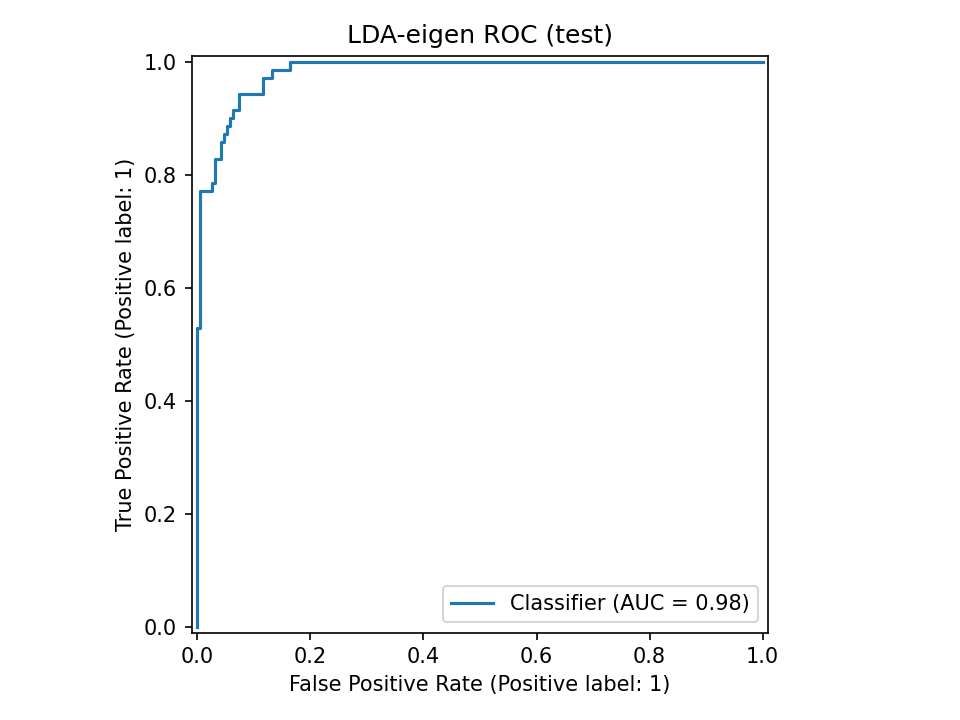
\includegraphics[width=.72\linewidth]{assets/LDA-eigen_roc_test.png}
	\caption{ROC curve on the test set (AUC $\approx 0.98$).}
	\label{fig:lda-roc}
\end{figure}

\begin{figure}[H]
	\centering
	\begin{subfigure}{.48\linewidth}
		\centering
		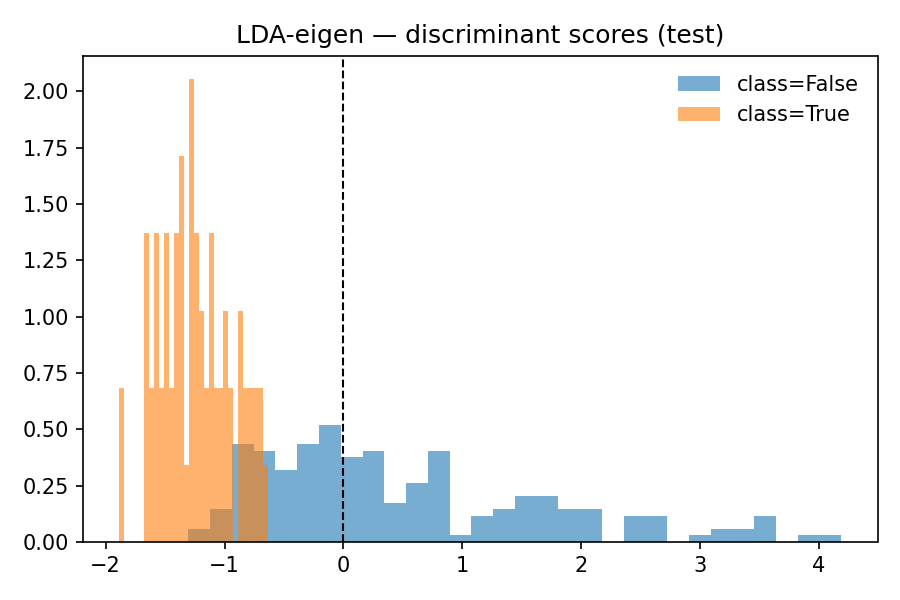
\includegraphics[width=\linewidth]{assets/LDA-eigen_scores_hist_test.png}
		\caption{LD1 scores (test).}
		\label{fig:lda-scores}
	\end{subfigure}\hfill
	\begin{subfigure}{.48\linewidth}
		\centering
		% Use your exported heatmap; if not available, replace with the numeric matrix figure.
		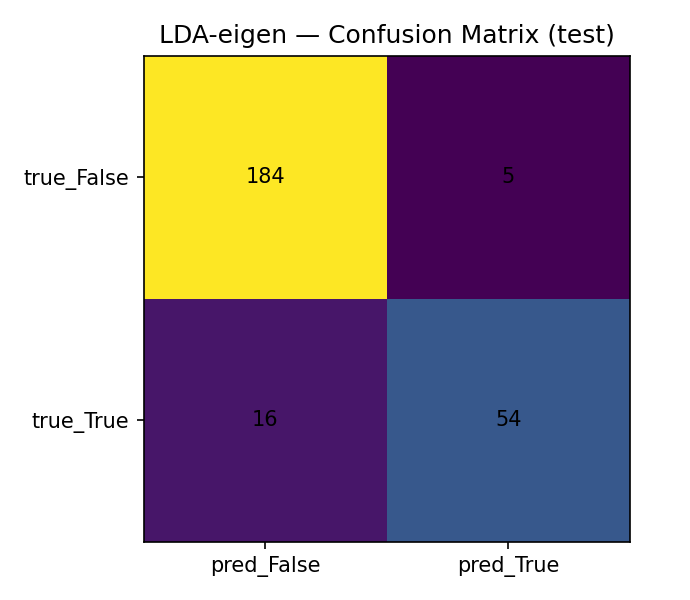
\includegraphics[width=\linewidth]{assets/LDA-eigen_confusion_test_heatmap.png}
		\caption{Confusion matrix (test).}
		\label{fig:lda-cm}
	\end{subfigure}
	\caption{Geometric separation and error structure. The dashed line in \subref{fig:lda-scores} marks the default decision boundary.}
	\label{fig:lda-geom}
\end{figure}

\begin{figure}[H]
	\centering
	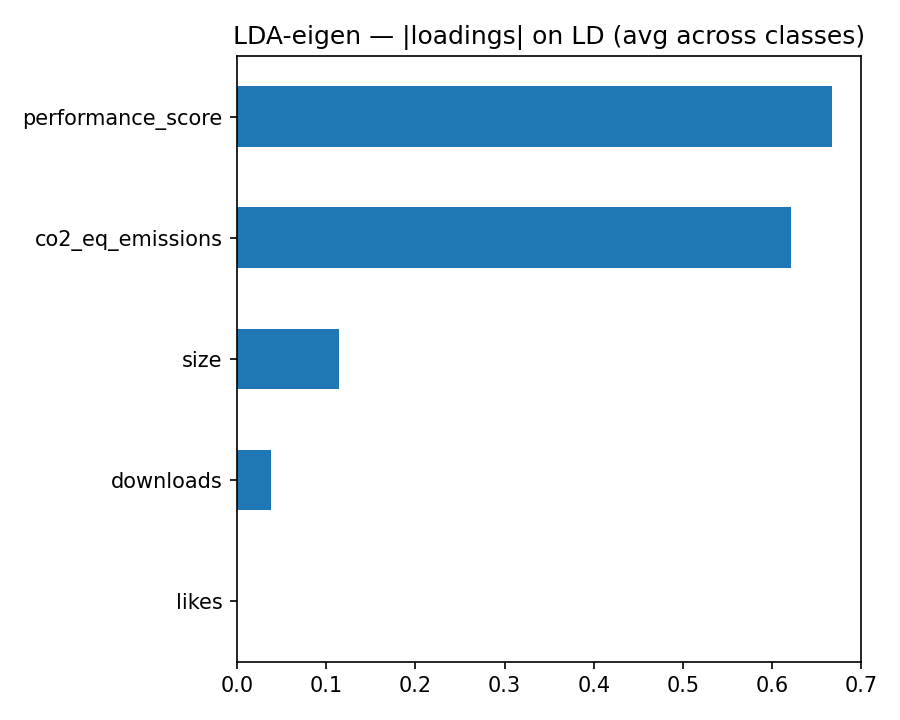
\includegraphics[width=.72\linewidth]{assets/LDA-eigen_loadings_abs_bar.png}
	\caption{Absolute loadings on LD1 (averaged across classes). Performance and CO$_2$ dominate; size and downloads are secondary; likes is negligible.}
	\label{fig:lda-loadings}
\end{figure}


\subsection{Results and Discussion}
Table~\ref{tab:clf-compare} summarizes the out-of-sample performance. The linear
baseline (LDA) achieved strong discrimination (AUC $=0.983$) with solid AP for the
minority class (AP$_{\text{True}}=0.958$) and good accuracy ($0.919$). The
non-linear models improved upon the baseline: SVM–RBF reached AUC $=0.991$,
AP$_{\text{True}}=0.979$, and Accuracy $=0.954$, with a Brier score of $0.033$
(acceptable calibration). Gradient Boosting performed best across all metrics with
AUC $=1.000$, AP$_{\text{True}}=1.000$, F1$_{\text{True}}=1.000$,
Accuracy $=1.000$, and a very low Brier score ($2.3\times10^{-5}$), consistent with
near-perfect separability on the test fold.

The precision–recall panels in Fig.~\ref{fig:pr-nonlinear} show uniformly higher
precision at a given recall for Gradient Boosting, while the confusion matrices in
Fig.~\ref{fig:cm-nonlinear} reveal zero errors for GB on this hold-out, in contrast
to a small number of false negatives for SVM–RBF. These gains, together with the
excellent calibration (low Brier), support GB as the top performer on this dataset.
Because perfect test scores can occasionally arise from random favorability,
additional repeated or nested CV is recommended to rule out accidental overfitting
and to confirm the robustness of the selection. In operational settings, decision
thresholds can be tuned on the calibrated probabilities to trade specificity for
sensitivity when detecting the positive (``fair'') class is mission-critical.


\begin{table}[H]
	\centering
	\sisetup{table-number-alignment=center, round-mode=places, round-precision=3, table-format=1.5}
	\caption{Test performance and  accuracy cross-validated (CV). AP is Area Precision Recall}
	\label{tab:perf-all}
	\begin{threeparttable}
		\begin{tabular}{l SS S S S}
			\toprule
			\multirow{2}{*}{\textbf{Model}} & \multicolumn{2}{c}{\textbf{AUC}} & \textbf{AP\textsubscript{True}} & \textbf{F1\textsubscript{True}} & \textbf{Accuracy} \\
			\cmidrule(lr){2-3}
			& {\textbf{CV}} & {\textbf{test}} & & & \\
			\midrule
			LDA       & 0.925   & 0.983   & 0.958   & 0.837   & 0.919 \\
			SVM--RBF  & 0.98793 & 0.99127 & 0.97885 & 0.91177 & 0.95367 \\
			GradBoost & 0.99994 & 1.00000 & 1.00000 & 1.00000 & 1.00000 \\
			\bottomrule
		\end{tabular}
	\end{threeparttable}
\end{table}


\begin{figure}[H]
	\centering
	\begin{subfigure}{.48\linewidth}
		\centering
		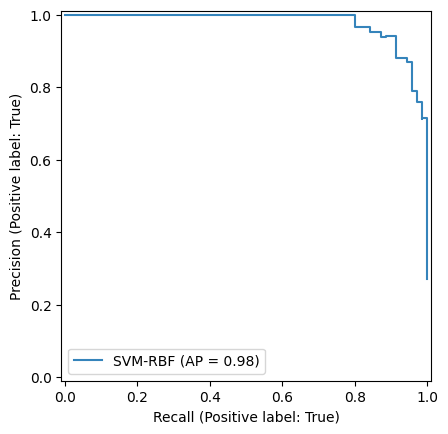
\includegraphics[width=\linewidth]{assets/svm_pr.png}% <- replace with your path
		\caption{SVM--RBF (AP $\approx$ 0.98)}
	\end{subfigure}\hfill
	\begin{subfigure}{.48\linewidth}
		\centering
		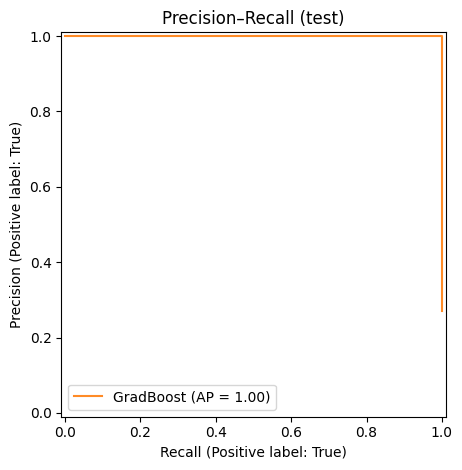
\includegraphics[width=\linewidth]{assets/gb_pr.png}% <- replace with your path
		\caption{Gradient Boosting (AP $\approx$ 1.00)}
	\end{subfigure}
	\caption{Precision--Recall curves on the test set for the positive class (\emph{True}).}
	\label{fig:pr-nonlinear}
\end{figure}

\begin{figure}[H]
	\centering
	\begin{subfigure}{.48\linewidth}
		\centering
		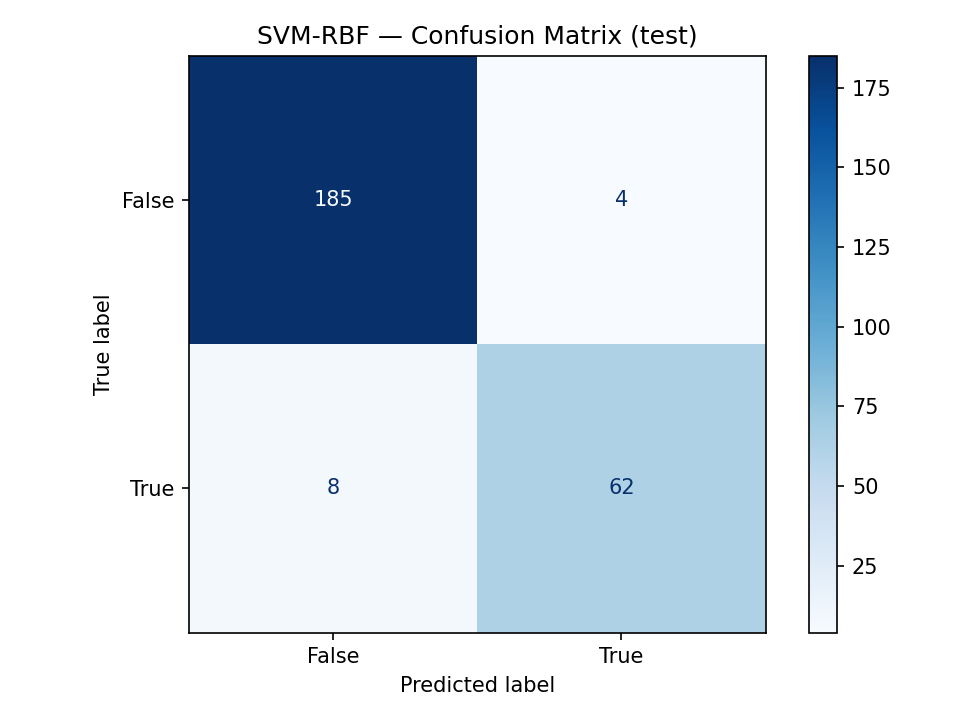
\includegraphics[width=\linewidth]{assets/cm_svmrbf_test.png}% <- replace with your path
		\caption{SVM--RBF}
	\end{subfigure}\hfill
	\begin{subfigure}{.48\linewidth}
		\centering
		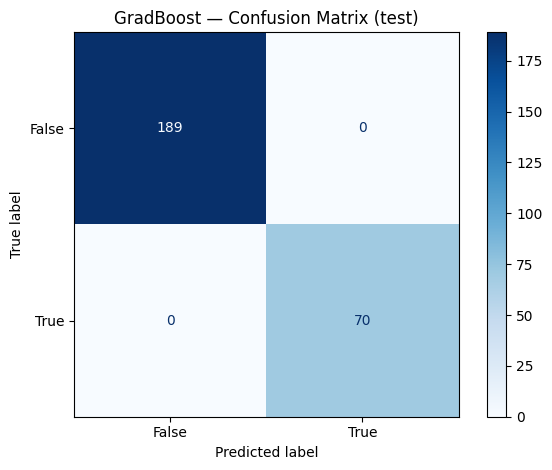
\includegraphics[width=\linewidth]{assets/gb_cm.png}% <- replace with your path
		\caption{Gradient Boosting}
	\end{subfigure}
	\caption{Confusion matrices on the held-out test set.}
	\label{fig:cm-nonlinear}
\end{figure}

\paragraph{Recommendation.}
Gradient Boosting is recommended as the primary model given its dominant AUC, AP,
F1, accuracy, and calibration. SVM–RBF is a strong runner-up and may be preferable
when model simplicity or margin-based robustness is desired. LDA remains valuable
as an interpretable baseline and for feature understanding via discriminant loadings.
	\section{Conclusions}
	\label{sec:conclusion}


	\bibliographystyle{IEEEtran}

	\bibliography{mybibfile}
\end{document}